\subsection*{Problema 4b}

Interpola la curva paramétria de la ecuación \ref{eq:ft_problma4b}.

\begin{equation}
	f(t) = (r(t)sin(t),r(t)cos(t)) \label{eq:ft_problma4b}
\end{equation}

donde

\begin{equation*}
	r(t) = exp(cos(t)-2cos(4t)+sin\left (\frac{t}{12}\right )^5
\end{equation*}

a partir de 25 puntos definidos en la ecuación \ref{eq:points_4b}.

\begin{equation}
	(x_i,y_i) = (x(t_i),y(t_i)) \qquad t_i = \frac{\pi i}{12} \qquad i=0,1,2,\dots,24 \label{eq:points_4b}
\end{equation}

\begin{figure}[H]
	\centering
	\begin{subfigure}[b]{7cm}
		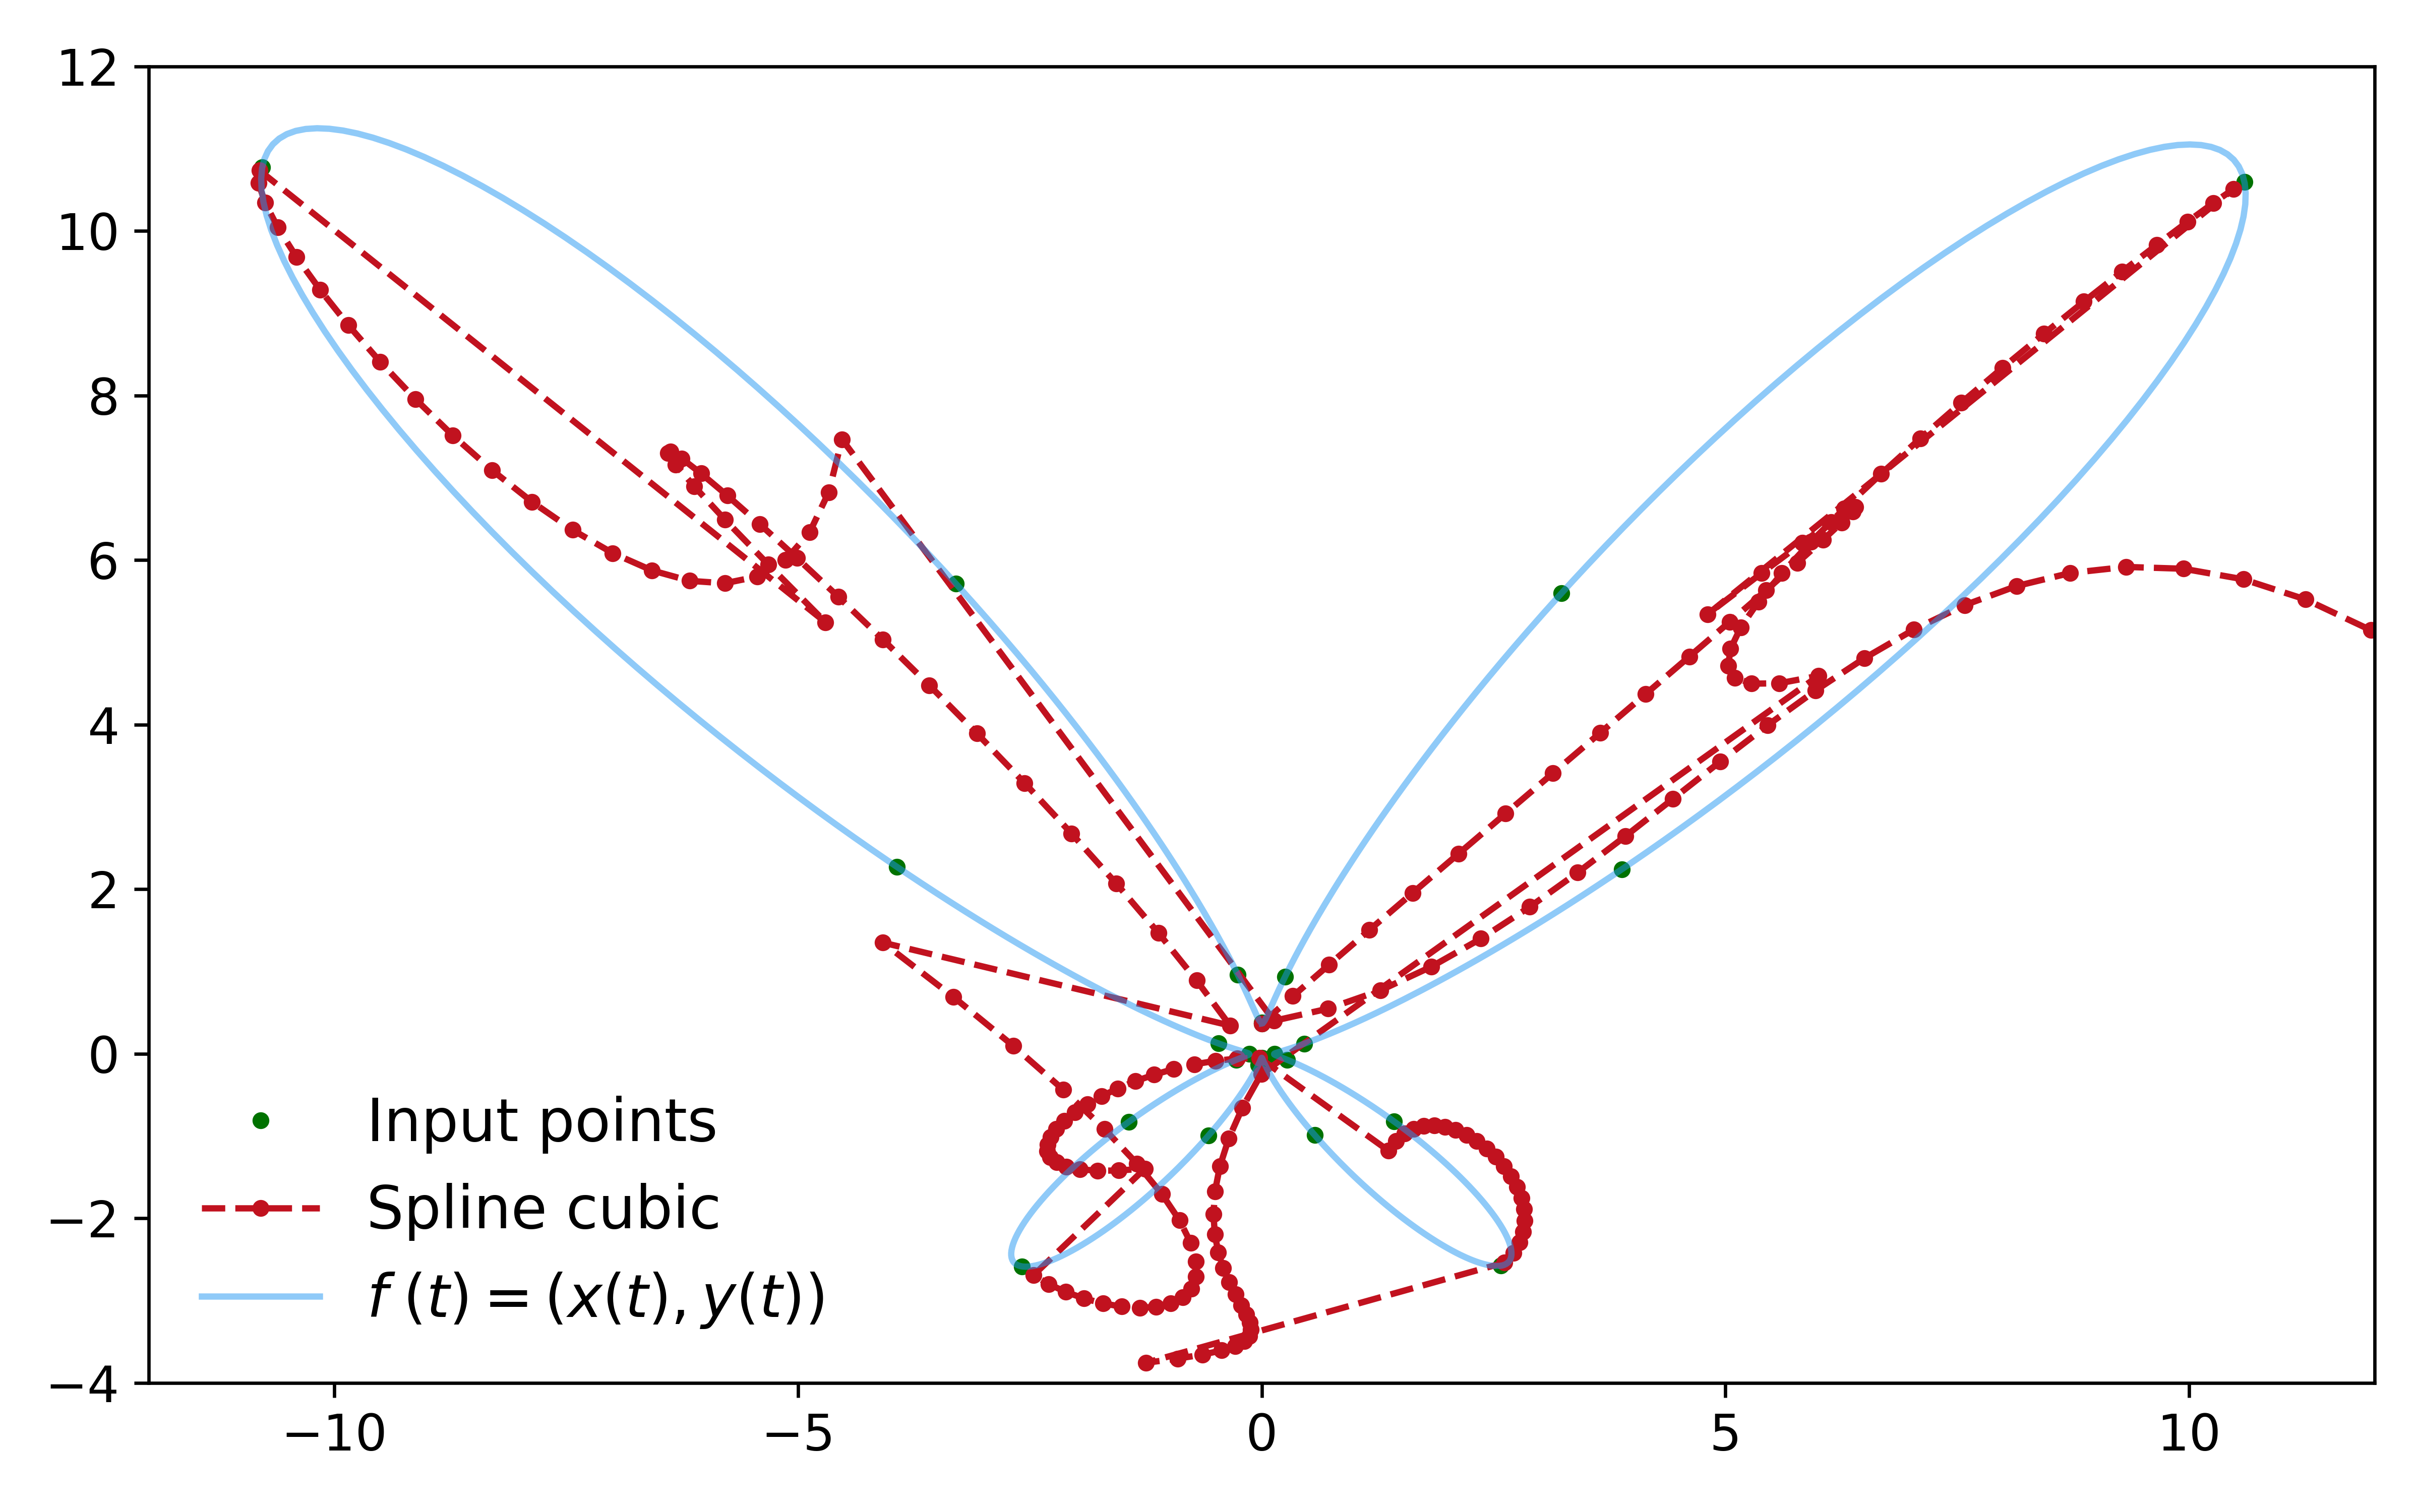
\includegraphics[width=7cm]{Graphics/problema04b_10.png}
		\caption{}
	\end{subfigure}
	\begin{subfigure}[b]{7cm}
		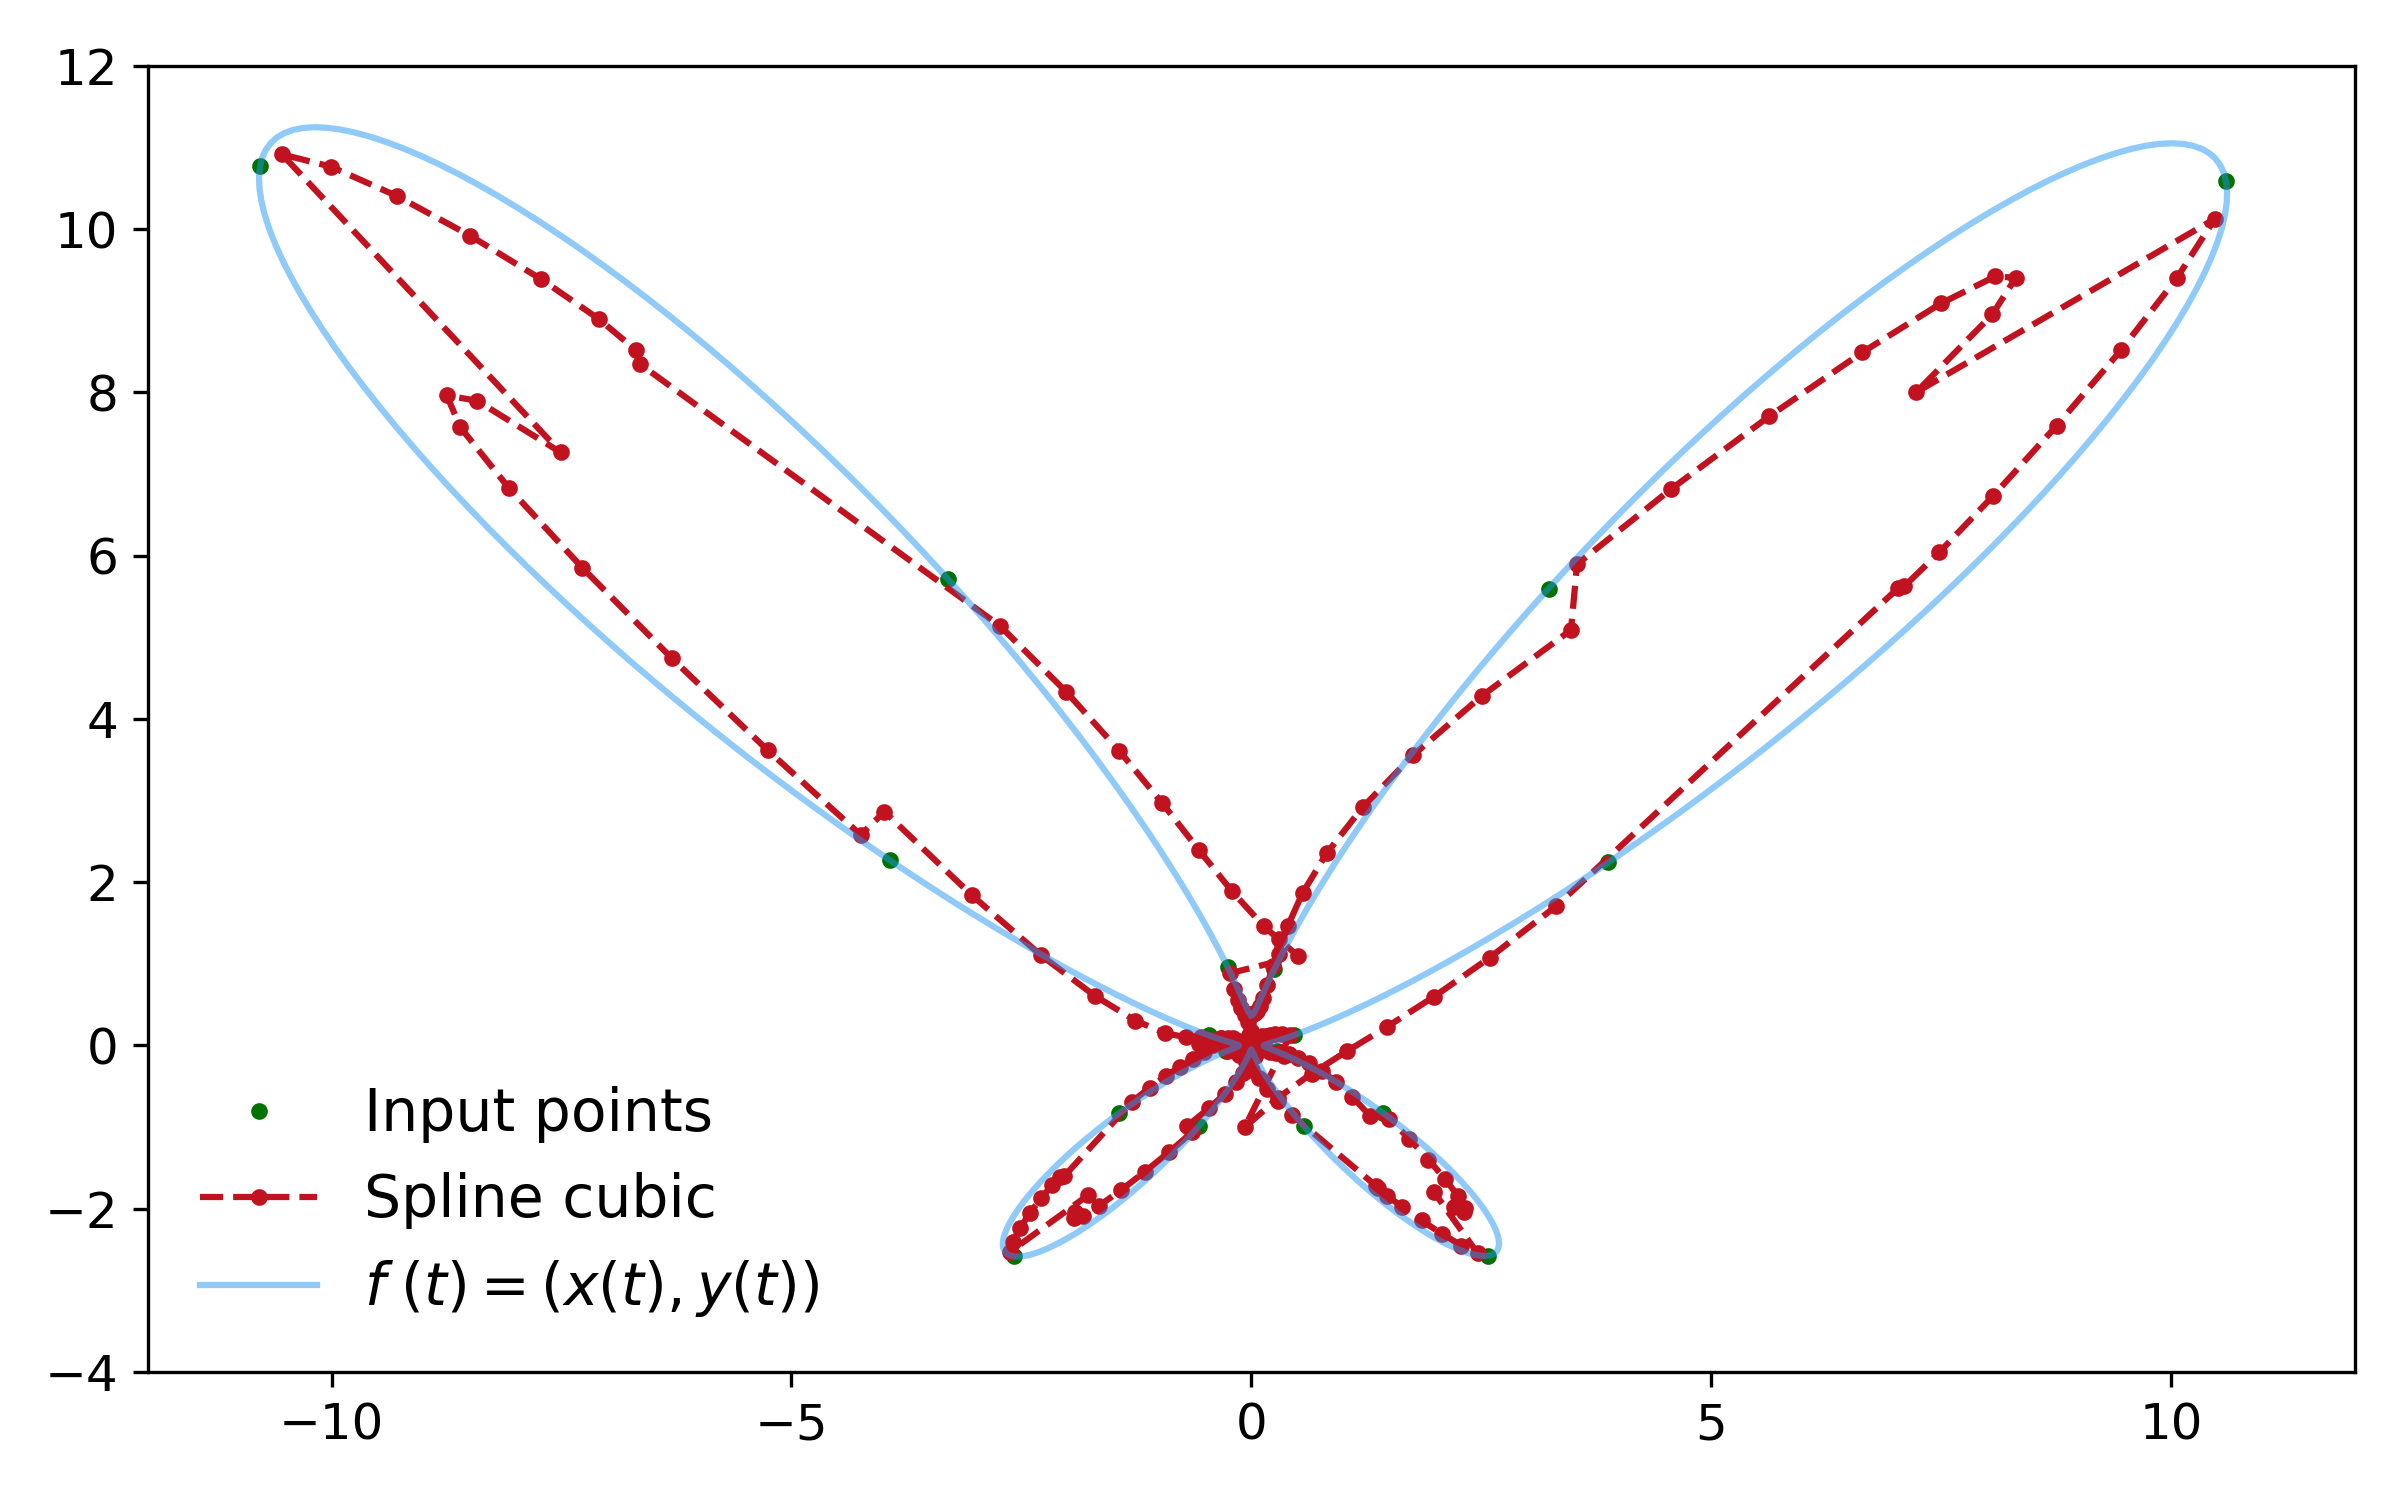
\includegraphics[width=7cm]{Graphics/problema04b_25.png}
		\caption{}
	\end{subfigure}
	\begin{subfigure}[b]{7cm}
		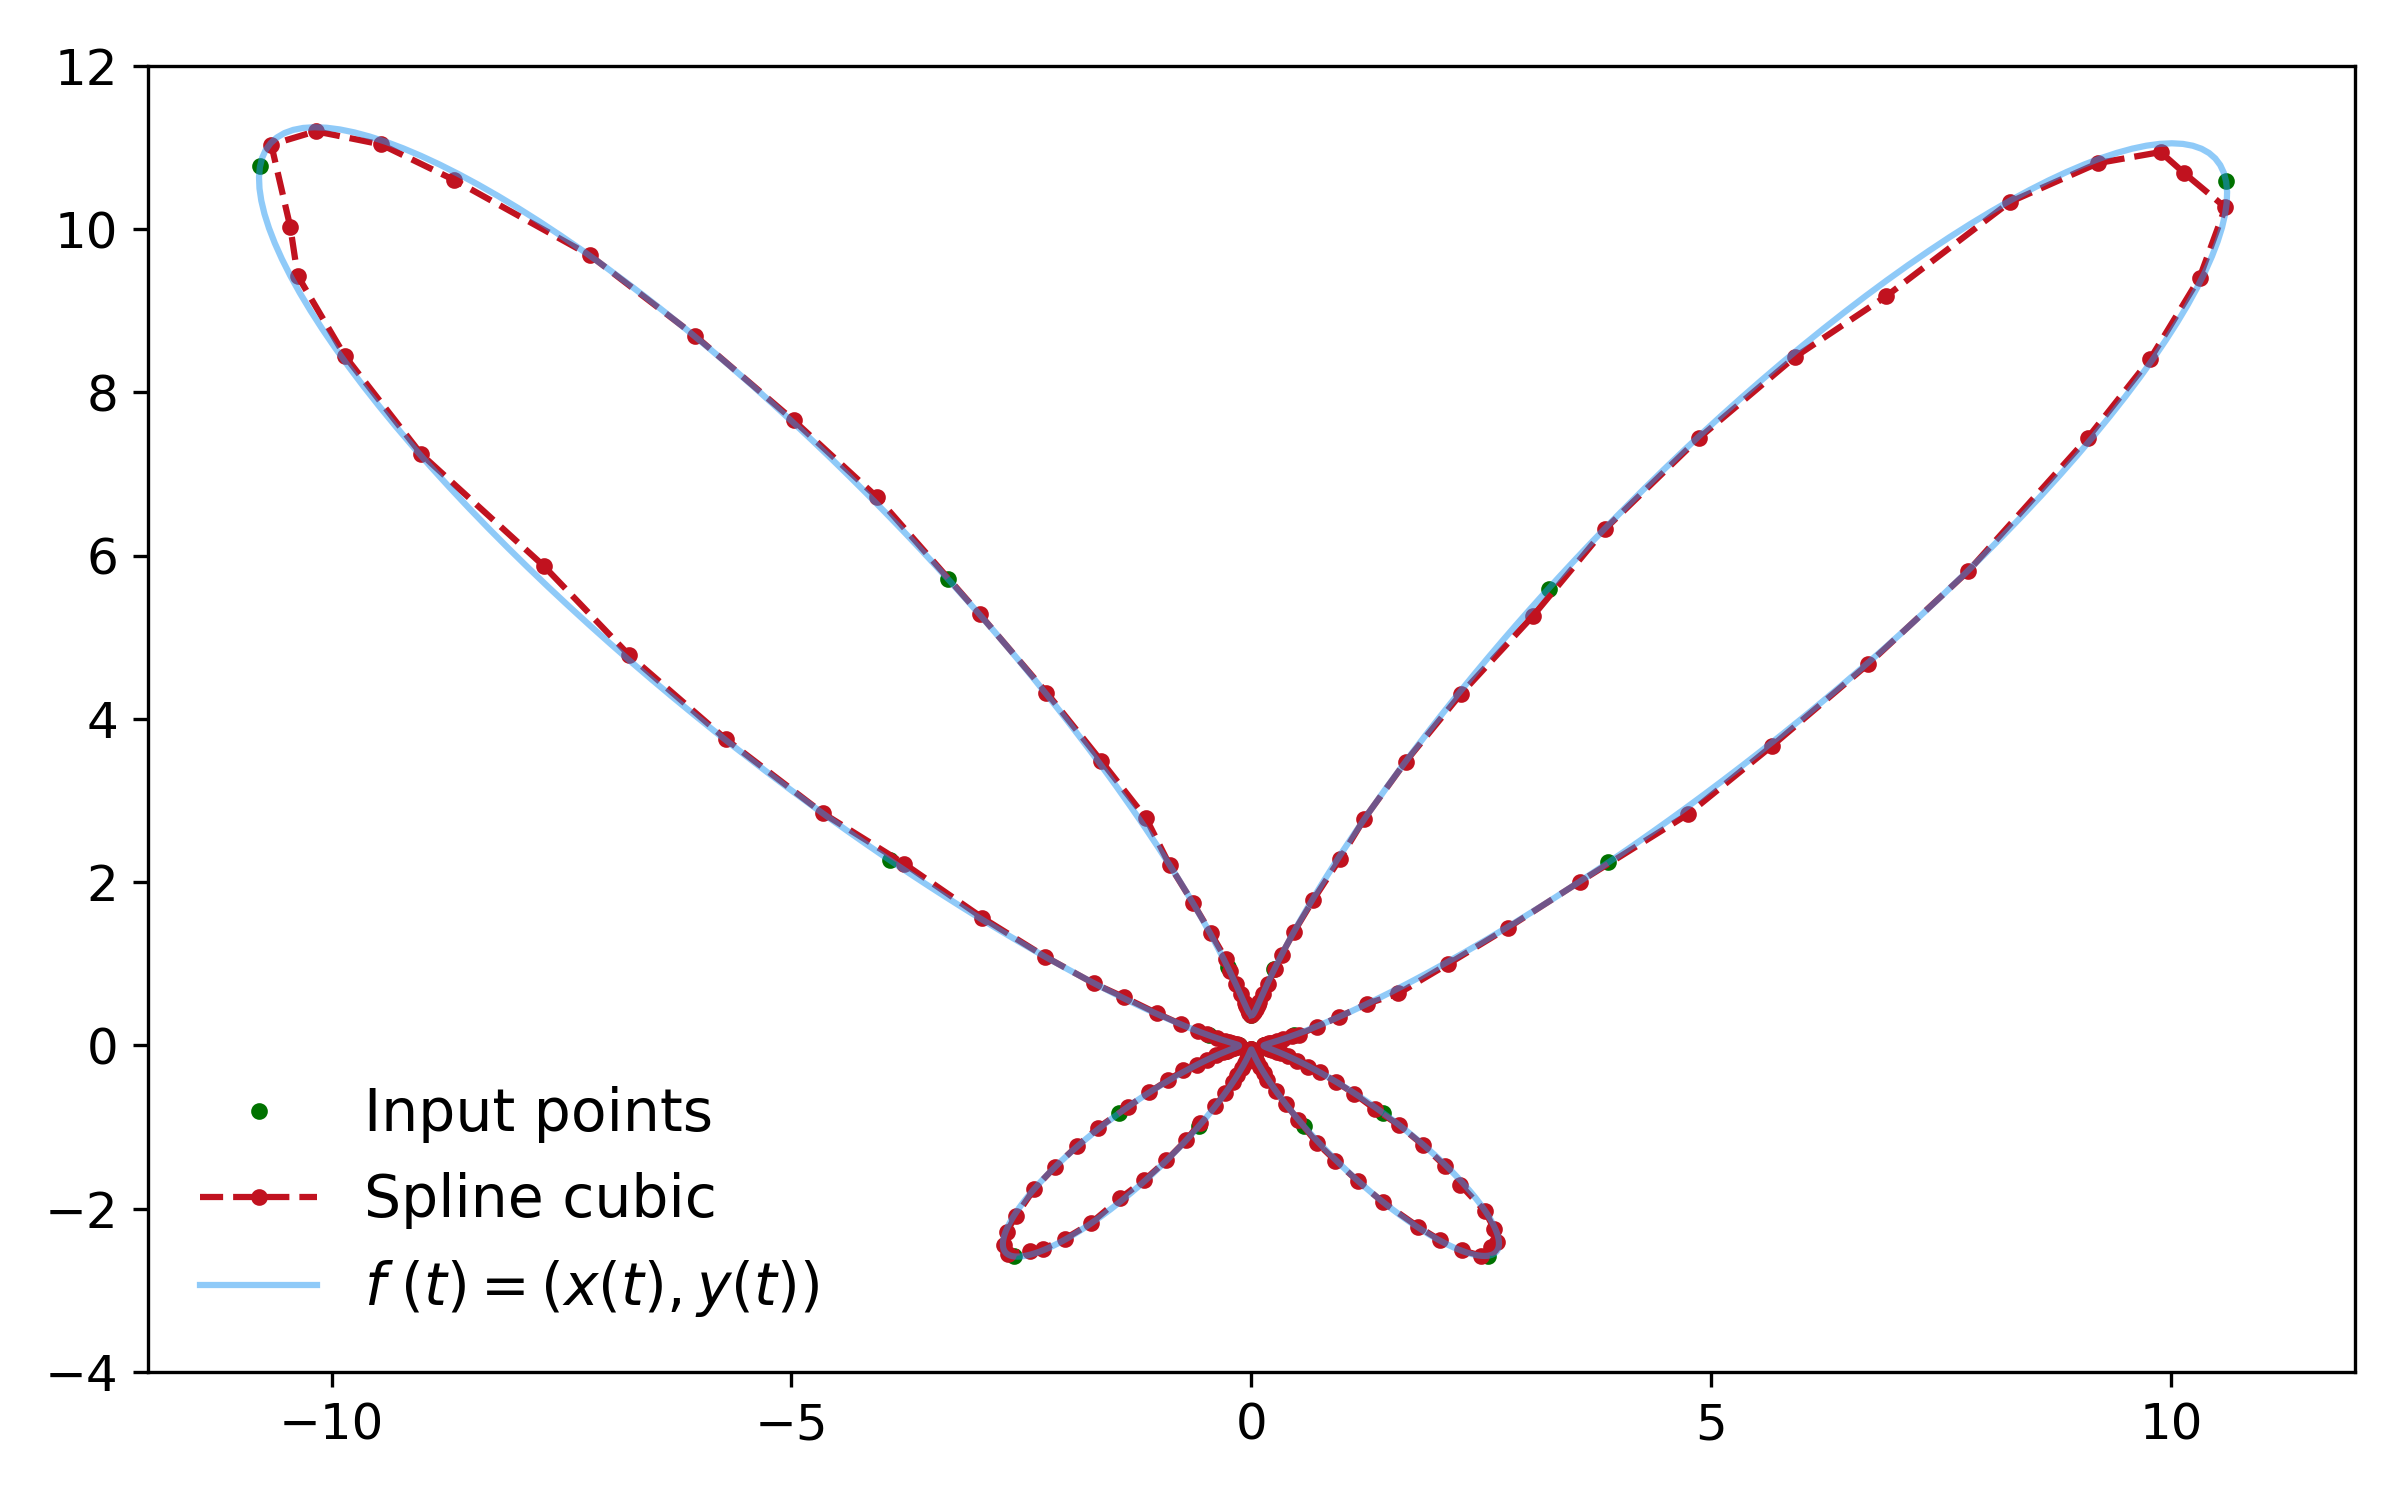
\includegraphics[width=7cm]{Graphics/problema04b_50.png}
		\caption{}
	\end{subfigure}
	\begin{subfigure}[b]{7cm}
		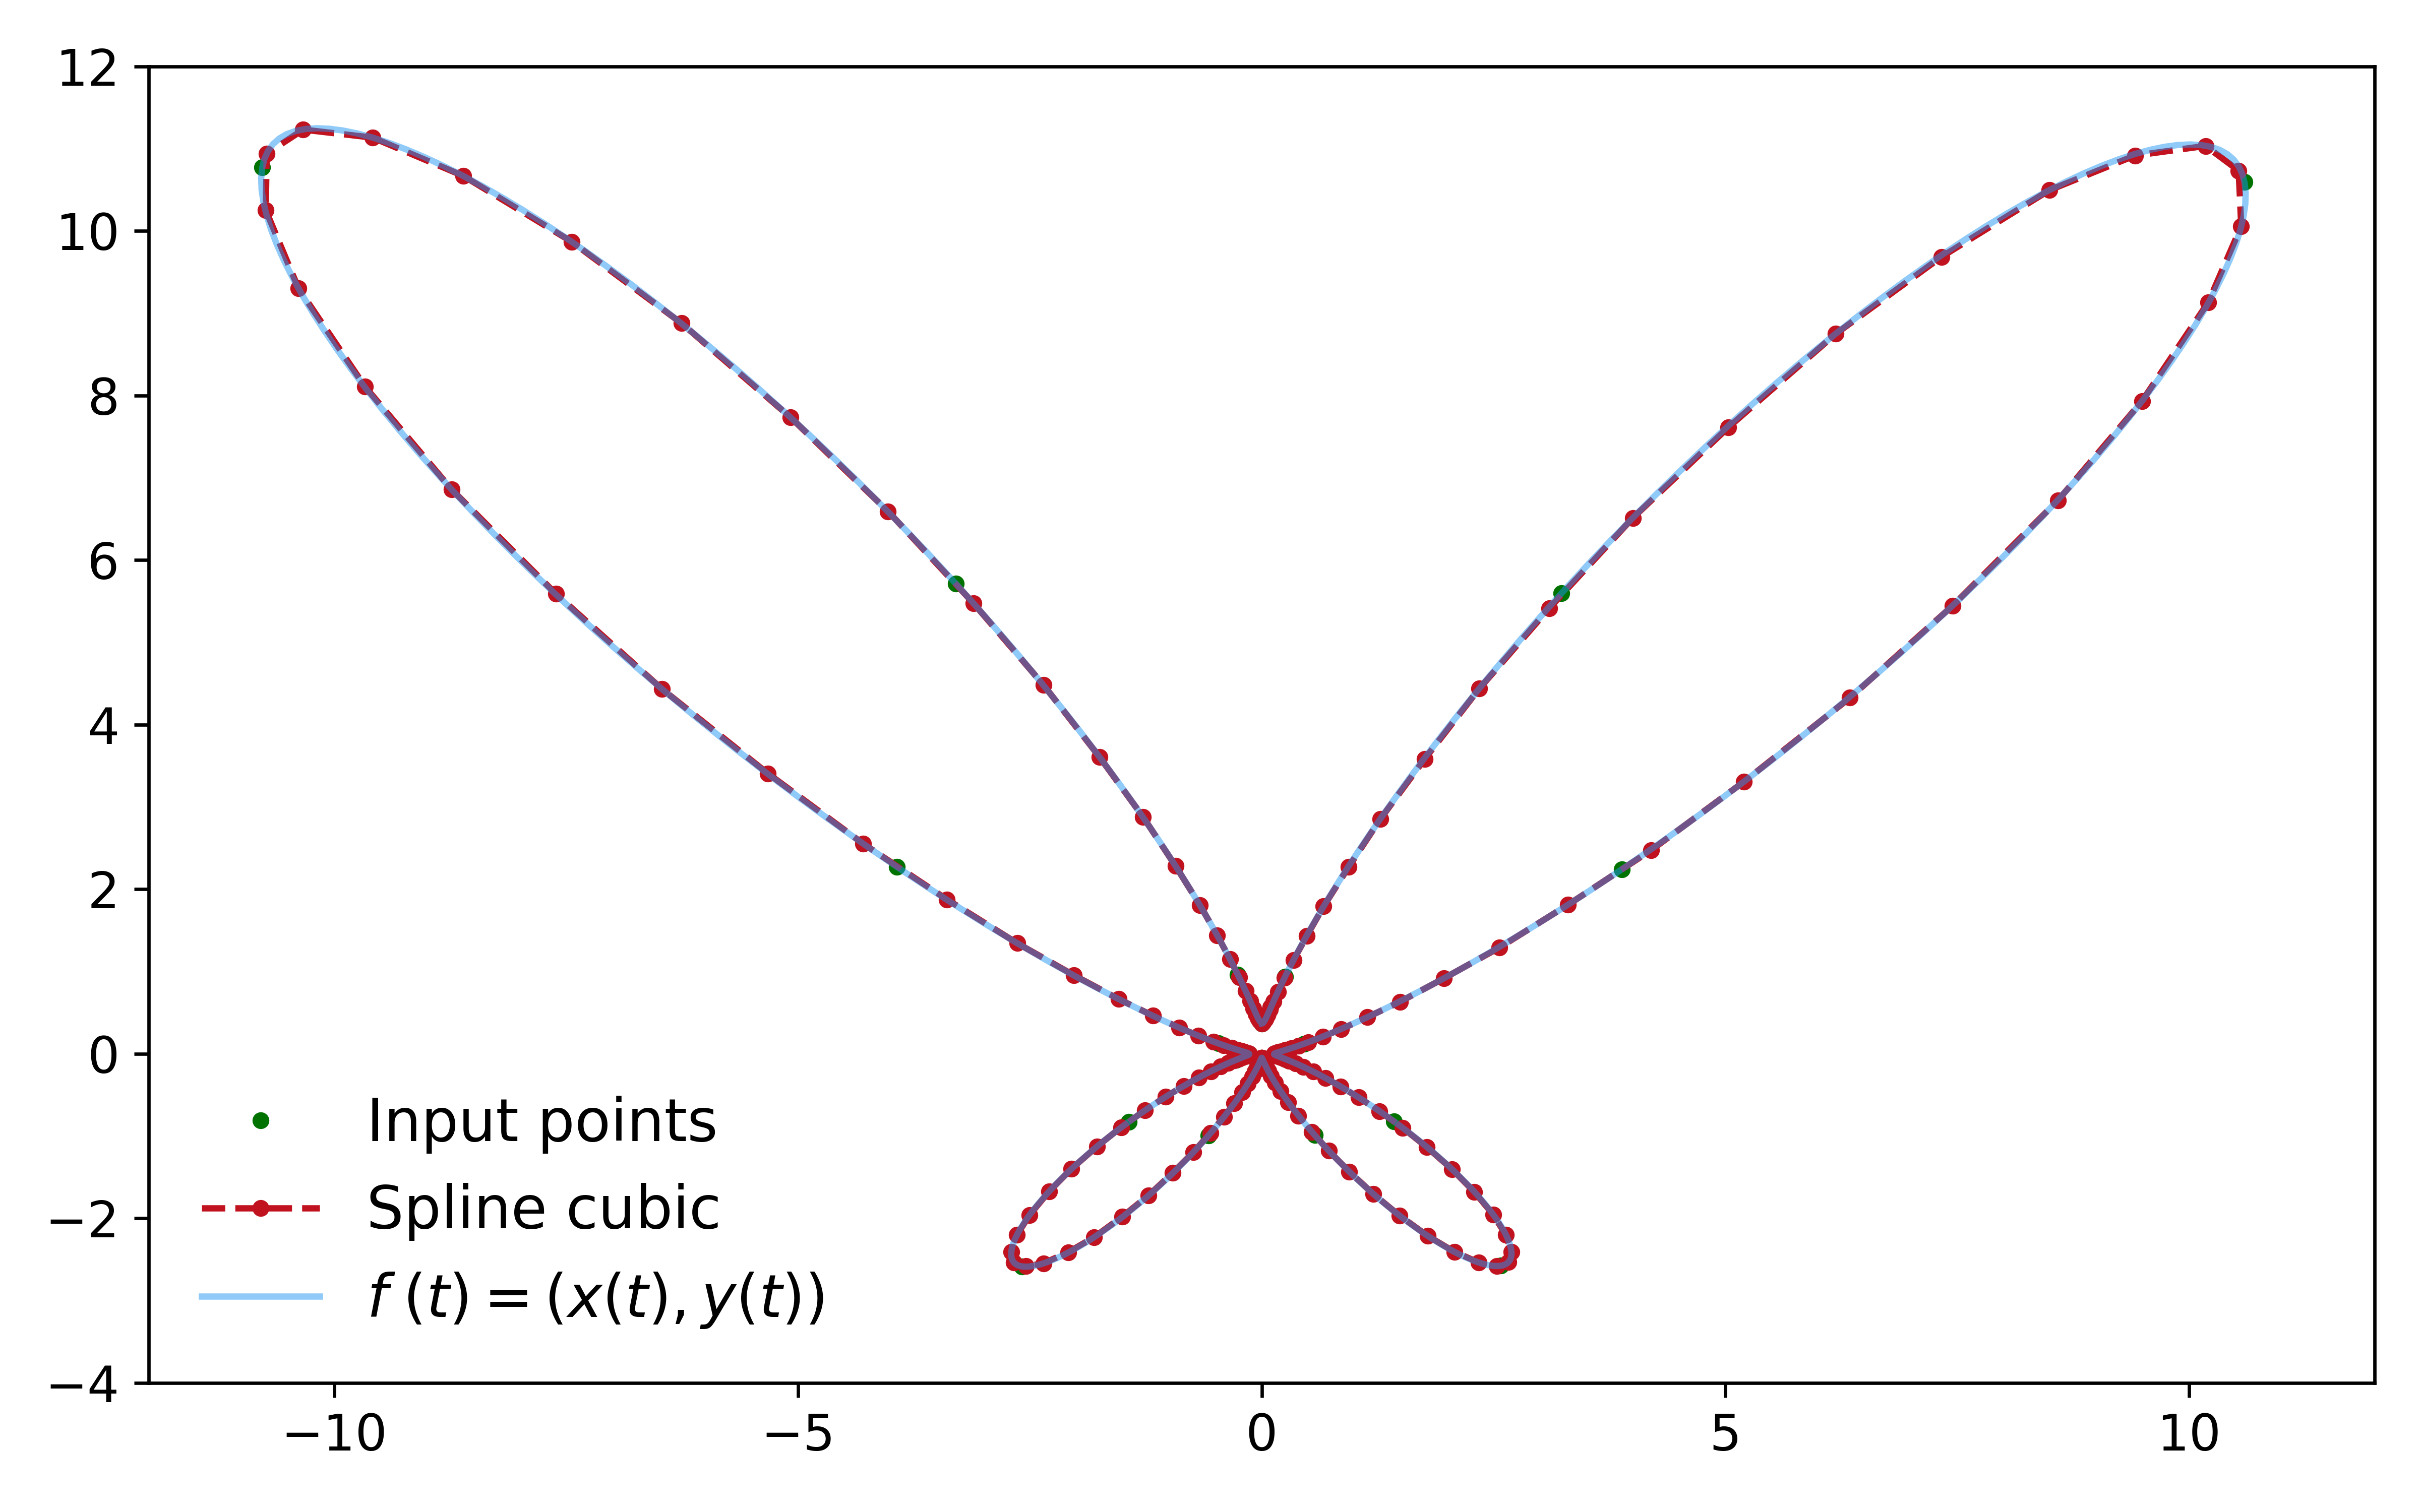
\includegraphics[width=7cm]{Graphics/problema04b_100.png}
		\caption{}
	\end{subfigure}
	\caption{}
\end{figure}
\pagebreak
